\section{Literatür verisiyle yazılım uygulamaları}
\label{sec:spss-b03}

\textbf{Amaç ve veri.} \texttt{b03.csv} içindeki not ve devamsızlık
sayısının merkezini ve yayılımını birlikte okuyun \citep{cortez2008data}.


\textbf{Ortak veri.} \nolinkurl{companion/spss/csv/b03.csv} ile B01
pilot paketindeki \texttt{b01.csv} bayt düzeyinde aynıdır. Paylaşılan
B03 uygulamasında R ve Python mevcut \texttt{b01.csv} dosyasını, SPSS
ise B01 CSV içe aktarımında kaydedilen \texttt{b01.sav} dosyasını
kullanmıştır. Aynı 395 kayıt yeniden incelenmektedir; yeni bir bağımsız
örneklem söz konusu değildir. Bu karşılaştırma Excel içe aktarmanın
doğrulandığı anlamına gelmez. Kodları \texttt{companion} klasörünü
içeren paket kökünden çalıştırın; veri sözlüğü ve hazırlık için bkz.
sayfa~\pageref{sec:spss-guide}.

\subsection{IBM SPSS uygulaması}
\textbf{Başlamadan önce.} Doğrulanan CSV yolunu izlemek için B01
verisini açan \texttt{open-b01.sps} dosyasını çalıştırın; bu işlem
\texttt{b01.sav} dosyasını yeniden oluşturur. Aşağıdaki tam blok da
aynı hazırlığı yapıp etiketli dosyayı açar; menü yolu alternatif uygulamadır.

\begin{spssadimlar}
\spssadim{\emph{Analyze $\to$ Descriptive Statistics $\to$ Explore} yolunu açın.}
\spssadim{\texttt{g3} ve \texttt{absences} değişkenlerini \emph{Dependent List} alanına taşıyın; \emph{Factor List} boş kalsın. \emph{Display} için \emph{Both} seçin.}
\spssadim{\emph{Statistics} içinde \emph{Descriptives} seçili, ortalama güven düzeyi yüzde 95 olsun; \emph{Continue} seçin.}
\spssadim{\emph{Plots} içinde \emph{Histogram} seçin; kutu grafiklerini etkin bırakın, yalnız bu grafikler isteniyorsa \emph{Stem-and-leaf} seçimini kaldırın. \emph{Continue $\to$ OK} ile çalıştırın.}
\spssadim{Ayrı medyan kontrolü için \emph{Analyze $\to$ Descriptive Statistics $\to$ Frequencies} yolunda \texttt{g3} seçin. \emph{Statistics $\to$ Median}, ardından \emph{Continue $\to$ OK} seçin.}
\end{spssadimlar}

{\raggedright
\noindent\textbf{Komutların görevi.} \texttt{EXAMINE} grafiklerle betimsel özetleri birlikte üretir; \texttt{CINTERVAL=95} ortalamanın güven düzeyidir. Son \texttt{FREQUENCIES} komutu medyanı ayrıca listeler.\par}

\par\noindent\begin{minipage}{\linewidth}
\textbf{Uygulama kodu:} \texttt{b03}. Doğrulanan pilotun veri dosyası:
\texttt{sav/b01.sav} (\texttt{companion/spss} altında).

\begin{lstlisting}[style=prismSPSS]
INSERT FILE='companion/spss/syntax/open-b01.sps'
 ERROR=STOP.
GET FILE='companion/spss/sav/b01.sav'.
FILTER OFF.
WEIGHT OFF.
SPLIT FILE OFF.
EXAMINE VARIABLES=g3 absences
 /PLOT=BOXPLOT HISTOGRAM
 /STATISTICS=DESCRIPTIVES /CINTERVAL=95.
FREQUENCIES VARIABLES=g3 /STATISTICS=MEDIAN.
\end{lstlisting}

\end{minipage}\par

\begin{outputguidebox}
\textbf{Paylaşılan SPSS çıktısıyla doğrulanan değerler.}
Notlar için ortalama \SPMatMean, medyan \SPMatMedian\ ve standart sapma
\SPMatSD\ bulunmuştur. \texttt{absences} ortalaması \SPAbsMean, standart sapması
\SPAbsSD, en yüksek değeri 75'tir. Histogram ve kutu grafiği, tek bir
ortalamanın gizlediği sıfırları ve sağ kuyruğu inceleme olanağı sağlar.
Bir kutu grafiği işareti otomatik veri silme kararı değildir: örneğin
devamsızlık değeri 75 olan kayıt kaynağa dönülerek araştırılmalıdır.
Notlardaki 38 sıfır korunmuştur.
\end{outputguidebox}


\par\noindent\begin{minipage}{\linewidth}
\subsection{R uygulaması}
\label{sec:r-gercek-b03}

\texttt{sd} örneklem standart sapmasını, \texttt{median} medyanı hesaplar. \texttt{conf.int} yalnız ortalama aralığını seçer; bu uygulamada test sonucu yorumlanmaz.

\begin{lstlisting}[style=prismR]
d <- read.csv("companion/spss/csv/b03.csv")
stopifnot(!anyNA(d))
print(sapply(d[c("g3", "absences")], function(v)
  c(n=length(v), mean=mean(v), sd=sd(v),
    median=median(v), min=min(v), max=max(v))))
print(t.test(d$g3, conf.level=.95)$conf.int)
print(t.test(d$absences, conf.level=.95)$conf.int)
par(mfrow=c(2, 2))
for (v in c("g3", "absences")) {
  hist(d[[v]], main=v, xlab=v)
  boxplot(d[[v]], main=v)
}
par(mfrow=c(1, 1))
\end{lstlisting}

\textbf{Çıktıyı okuma.} Paylaşılan R çıktısında 395 satır ve 10 sütun
vardır; tüm sütunların eksik değer sayımları sıfırdır. \texttt{n},
\texttt{mean}, \texttt{sd}, \texttt{median}, \texttt{min} ve
\texttt{max} satırlarını ortak tabloyla eşleştirin. Her iki değişkenin
ortalaması için yüzde 95 güven aralığı ayrıca doğrulanmıştır.
\end{minipage}\par

\par\noindent\begin{minipage}{\linewidth}
\subsection{Python uygulaması}
\label{sec:python-b03}

\texttt{std} örneklem standart sapmasıdır. \texttt{confidence\_interval} ortalama aralığını verir; burada sıfır ortalamasına karşı test yapmak amaçlanmaz.

\begin{lstlisting}[style=prismPythonApp]
import pandas as pd
import numpy as np
from scipy import stats
import matplotlib.pyplot as plt

d = pd.read_csv("companion/spss/csv/b03.csv")
assert not d.isna().any().any()
print(d[["g3", "absences"]].agg(
    ["count", "mean", "std", "median", "min", "max"]))
print(stats.ttest_1samp(d.g3, 0).confidence_interval(.95))
print(stats.ttest_1samp(d.absences, 0).confidence_interval(.95))
fig, axes = plt.subplots(2, 2)
for row, v in enumerate(["g3", "absences"]):
    axes[row, 0].hist(d[v], bins=15)
    axes[row, 0].set_title(v)
    axes[row, 1].boxplot(d[v]); axes[row, 1].set_title(v)
plt.tight_layout(); plt.show()
\end{lstlisting}

\textbf{Çıktıyı okuma.} Paylaşılan Python çıktısında da 395 satır,
10 sütun ve her sütunda sıfır eksik değer görülür. \texttt{count}
R'deki \texttt{n}, \texttt{std} ise \texttt{sd} satırına karşılık gelir.
Paylaşılan kontrol betiği aralıkları doğrudan \texttt{stats.t.interval}
ile hesaplamıştır; yukarıdaki kod aynı tek örneklem $t$ aralığını verir.
Bu uygulamada sıfır ortalamasına karşı bir test sonucu yorumlanmaz.
\end{minipage}\par

\subsection{Sonuçların karşılaştırılması ve ortak rapor}
12 Eylül 2026'da paylaşılan SPSS tabloları ve grafikleri, R ve Python
metin çıktıları ve grafikleriyle karşılaştırılmıştır. İki değişkene ait
12 betimsel değer ile iki güven aralığının dört sınırı R ve Python'da
dokuz ondalık basamakta eşleşmiş; proje CSV'sinden yapılan hesaplar
ve SPSS'in yuvarlanmış değerleriyle de uyum sağlanmıştır.
Aşağıdaki tablolar doğrulanan çıktıların kitap düzenine uyarlanmış
özetidir; ekran görüntüsü değildir.

\begin{table}[H]
\centering
\caption{B03 verisinde not ve devamsızlığın doğrulanmış betimsel özetleri}
\label{tab:b03-dogrulanmis-betimsel}
\begin{tabular}{@{}lrr@{}}
\toprule
Ölçü & Yıl sonu notu & Devamsızlık sayısı \\
\midrule
Geçerli gözlem sayısı & 395 & 395 \\
Ortalama & 10,42 & 5,71 \\
Örneklem std. sapması & 4,581 & 8,003 \\
Medyan & 11 & 4 \\
En küçük değer & 0 & 0 \\
En büyük değer & 20 & 75 \\
\bottomrule
\end{tabular}
\par\smallskip
{\footnotesize Ortalamalar iki, standart sapmalar üç ondalık basamağa
yuvarlanmıştır. R ve Python çıktılarında yıl sonu notu sıfır olan
38 kayıt sayılmış; bu kayıtlar hesaplardan çıkarılmamıştır.\par}
\end{table}

\begin{table}[H]
\centering
\caption{B03 verisinde ortalamalar için doğrulanmış yüzde 95 güven aralıkları}
\label{tab:b03-dogrulanmis-aralik}
\begin{tabular}{@{}lrr@{}}
\toprule
Değişken & Alt sınır & Üst sınır \\
\midrule
Yıl sonu notu & 9,96 & 10,87 \\
Devamsızlık sayısı & 4,92 & 6,50 \\
\bottomrule
\end{tabular}
\par\smallskip
{\footnotesize Aralıklar $\bar{x}\pm t_{0{,}975;394}s/\sqrt{395}$
ile hesaplanmış ve iki ondalık basamağa yuvarlanmıştır.
Bunlar bireysel gözlemlerin değil, ortalamaların aralıklarıdır.\par}
\end{table}

\begin{figure}[H]
\centering
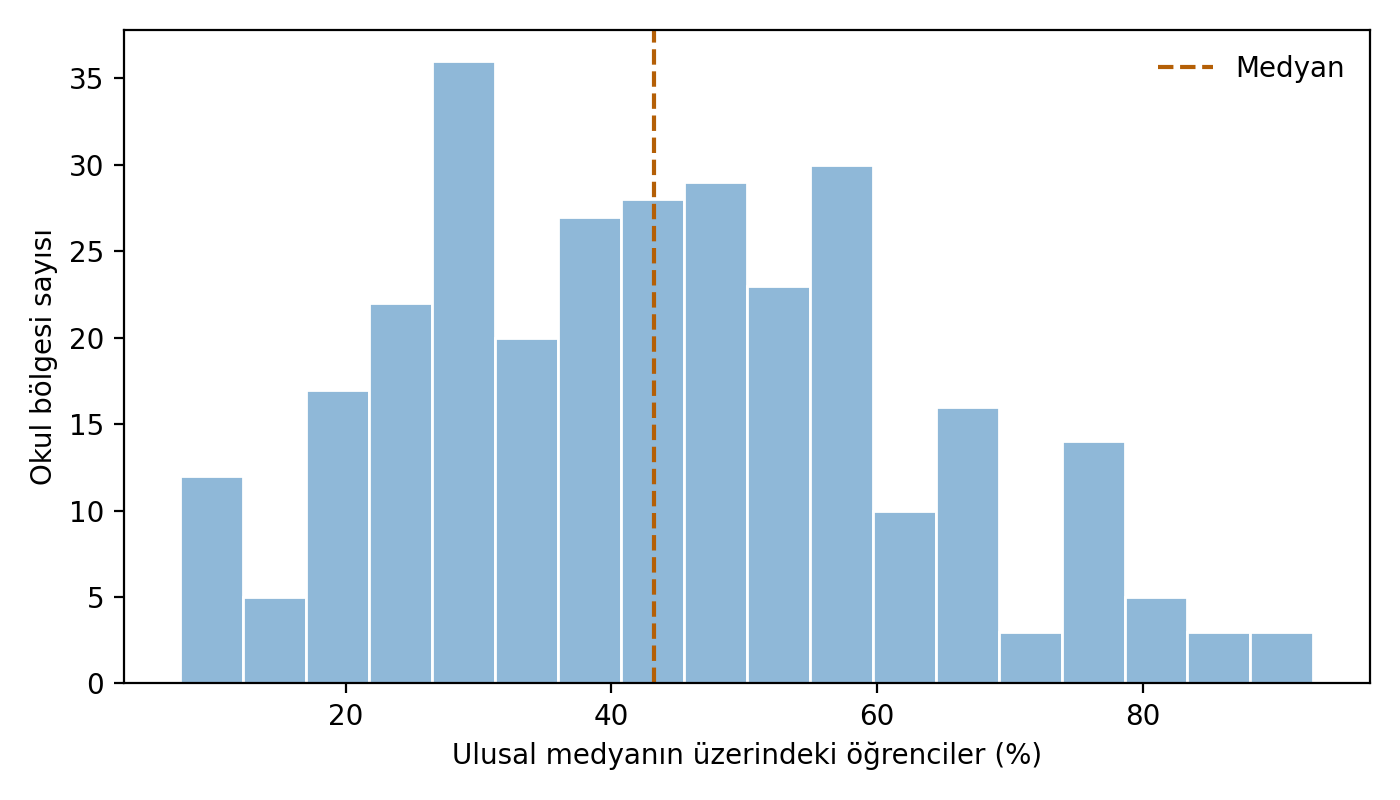
\includegraphics[width=\linewidth]{companion/outputs/figures/chapter03_star98_distribution.png}
\caption{B03 için paylaşılan Python histogramları ve kutu grafikleri.
Üst sıra yıl sonu notunu, alt sıra devamsızlık sayısını gösterir.}
\label{fig:b03-dogrulanmis-grafikler}
\end{figure}

\Needspace{22\baselineskip}
\begin{outputguidebox}
Tablo~\ref{tab:b03-dogrulanmis-betimsel} içinde not ortalaması 10,42,
medyanı 11'dir. Şekil~\ref{fig:b03-dogrulanmis-grafikler} içinde not
kutusunun sınırları 8 ve 14, bıyık uçları 0 ve 20'dir. Devamsızlık
dağılımında sağ kuyruk belirgindir; ortalama 5,71 iken medyan 4'tür.
Devamsızlık kutusu 0--8 aralığındadır; üst bıyık 20'ye uzanır,
daha yüksek değerler ayrı işaretlenir. Bu işaretler kayıtların hatalı
olduğunu tek başına göstermez.

Paylaşılan SPSS, R ve Python histogramlarının sınıf aralıkları farklı
olduğundan sütun yükseklikleri birebir eşleşmez. Karşılaştırılan kutu
grafiklerinde medyanlar, kutu sınırları ve bıyık uçları uyumludur;
işaret biçimleri ve gözlem etiketlerinin gösterimi farklıdır.
Hesapların uyumu örneklemin temsil gücünü kanıtlamaz.
Tablo~\ref{tab:b03-dogrulanmis-aralik} içindeki aralıkların daha geniş
bir evrene yönelik yorumu, örnekleme düzeni ve bağımsızlık gibi
çıkarım koşullarına bağlıdır; burada hesaplama uyumu doğrulanmıştır.
\end{outputguidebox}

\textbf{Raporlama örneği (doğrulanmış çıktılarla).}
``395 öğrencinin yıl sonu notu ortalaması 10,42, medyanı 11 ve standart
sapması 4,581 puandır. Devamsızlık sayısının ortalaması 5,71, medyanı 4
ve standart sapması 8,003'tür. Ortalama için hesaplanan yüzde 95
$t$ aralıkları sırasıyla 9,96--10,87 ve 4,92--6,50'dir. Sıfır notlu
38 kayıt korunmuş; devamsızlıkta 75'e ulaşan yüksek değerler grafiksel
incelemeye alınmış, otomatik olarak silinmemiştir. Sonuçlar daha geniş
bir öğrenci evrenine doğrudan genellenmemiştir.''


\textbf{Görev.} Not ve devamsızlık için birer grafik seçin. Aynı ölçeğe
sahip olmayan değişkenleri yalnız standart sapmalarını karşılaştırarak
``daha değişken'' ilan etmenin sakıncasını tartışın.